% ---------------------------------------------------------------
% Preamble
% ---------------------------------------------------------------
%\documentclass[a4paper,fleqn,longmktitle]{cas-sc}
\documentclass[a4paper,fleqn]{cas-dc}
%\documentclass[a4paper]{cas-dc}
%\documentclass[a4paper]{cas-sc}
% ---------------------------------------------------------------

% -------------------------------------------------------------------- 
% Packages
% --------------------------------------------------------------------
% Figure packages
\usepackage{float}
\usepackage{adjustbox}
% Text, input, formatting, and language-related packages
\usepackage[T1]{fontenc}
\usepackage{subcaption}
% \usepackage[utf8]{inputenc}
% \usepackage[nomath]{lmodern}

% Margin and formatting specifications
%\usepackage[authoryear]{natbib}
\usepackage[sort]{natbib}
\setcitestyle{square,numbers}

 %\bibliographystyle{cas-model2-names}

\usepackage{setspace}

% \usepackage[authoryear,longnamesfirst]{natbib}

% Math packages
\usepackage{amsmath, amsthm, amssymb, amsfonts, bm, nccmath, mathdots, mathtools, bigints, ulem}

% --------------------------------------------------------------------
% Packages Configurations
% --------------------------------------------------------------------
% (General) General configurations and fixes
\AtBeginDocument{\setlength{\FullWidth}{\textwidth}}	% Solves els-cas caption positioning issue
\setlength{\parindent}{20pt}
%\doublespacing
% --------------------------------------------------------------------
% Other Definitions
% --------------------------------------------------------------------

% --------------------------------------------------------------------
% Environments
% --------------------------------------------------------------------
% ...

% --------------------------------------------------------------------
% Commands
% --------------------------------------------------------------------

% ==============================================================
% ========================== DOCUMENT ==========================
% ==============================================================
\begin{document} 
%  --------------------------------------------------------------------

% ===================================================
% METADATA
% ===================================================
\title[mode=title]{Parameter estimation}                      
\shorttitle{Parameter estimation}

\shortauthors{A, B, C}

\author[1]{Oliwer Sliczniuk*}[orcid=0000-0003-2593-5956]
\ead{oliwer.sliczniuk@aalto.fi}
\cormark[1]
%\credit{a}

\author[1]{Pekka Oinas}[orcid=0000-0002-0183-5558]
%\credit{b}

\author[1]{Francesco Corona}[orcid=0000-0002-3615-1359]
%\credit{c}

\address[1]{Aalto University, School of Chemical Engineering, Espoo, 02150, Finland}
%\address[2]{2}

\cortext[cor1]{Corresponding author}

% ===================================================
% ABSTRACT
% ===================================================
\begin{abstract}
Given a system of partial differential equations, $F(t,x,\dot{x},p,u)=0$, where $x$ represents state variables, $p$ are the parameters, and $u$ are control variables, the process model is simultaneously solved for both $x_i$ and a set of sensitivity functions, $dx_i/dp_j$, overall times $t$.These sensitivity functions measure the influence of the parameter change on the model's output. As an example, the supercritical extraction process is presented. The impact of mass flow rate, pressure, and inlet temperature on the model's output is discussed. The sensitivity analysis results prove that the considered variables can affect the extraction's yield and be used as control variables in optimization problems. Moreover, the local sensitivity analysis results are analyzed from a phenomenological point of view to enhance understanding of the process model.

\end{abstract}

\begin{keywords}
Supercritical extraction \sep Parameter estimation \sep Mathematical modelling
\end{keywords}

% ===================================================
% TITLE
% ===================================================
\maketitle

% ===================================================
% Section: Introduction
% ===================================================\section{Introduction}

\section{Introduction}
%{\color{brown}Intro about extraction}\\
The extraction of natural substances from solid materials and liquids with solvents have been a popular subject of research and development in the last years. Supercritical fluids have multiple applications in an extraction process due to the pressure-dependent dissolving power and {\color{blue} both gas-and liquid-like properties (for example fluid-like density and gas-like diffusivity). Among different supercritical fluids, the supercritical $CO_2$ is one of the most popular due to it is nontoxic, non-flammable and non-corrosive properties. The critical point of $CO_2$ is relatively low ($73.8$ bar and $31 ^\circ C$), compare to other fluids. The supercritical extraction with $CO_2$ become attractive alternative, to replace traditional extraction techniques.}

%{\color{brown} Literature review of the models}\\
\sout{The supercritical extraction process is considered unconventional due to the lack of formulation of one general model, properties that strongly depend on working conditions and its unsteady nature. Understanding the physics behind the phenomena and the proper mathematical description is necessary to predict the process outcome. Several extraction models have been developed to characterize different mass transfer mechanisms and equilibrium relationships.}
{\color{blue}The extraction of valuable compounds from fixed bed of biomass can be described by one of many mathematical models as presented by \citet{Huang2012}. The selection the extraction model is not arbitrary and should be based on the knowledge of phenomenons occurring in the operational unit. Each model has its own assumptions and describe different mass transfer mechanisms and equilibrium relationships}. 

\citet{Reverchon1996} developed a model, which considers an oil as a single component and assumes that the extraction process is controlled by internal-mass transfer resistance. As a result of these assumptions, the external mass transfer was neglected. The original model of Reverchon does not consider the influence of axial dispersion and does not take into account the change of density and flow rate along the bed. 

Based on analogy to heat transfer, \citet{Reverchon1993} suggested a hot ball model, where the extraction process is treated analogously to {\color{blue} a process in which a hot ball is cooled in a uniform medium} \sout{the process of cooling down a hot ball in a uniform medium}. {\color{blue}The hot ball model is used to describe an extraction process from solid particles which contains small quantities of solute so that the solubility is not a limiting factor. }

\citet{Sovova1994} \sout{presented the Broken-and-Intact Cell model, which assumes the presence of two solid phases, the broken and intact cells. The results of applying Sovova's model allow distinguishing three phases of the extraction process (constant extraction rate, falling extraction rate, and diffusion-controlled periods) directly at the modelling stage.}
{\color{blue} presented the Broken-and-Intact Cell model. The BIC model describes a system where the outer surfaces of particles have been mechanically interrupted. The solute from the broken cells is easily accessible for the solvent. The extraction of easily accessible solute is fast and directly controlled by its diffusion and convection in the solvent.
However, the rest of the solute is less accessible because it is closed in the particle's core or intact cells. This solute slowly diffuses through the walls of a cell due to high mass transfer resistance.
In this model, the extraction process is divided into three periods controlled by different mass transfer mechanisms: Constant extraction rate (CER) period, Falling extraction rate (FER) period and Diffusion-controlled (DC) period.}

%{\color{brown}Methodology: sensitivity analysis }\\
As in many engineering problems, mathematical modelling is crucial to mimic real-life objects, but it requires knowing multiple parameter values. One way to better understand the phenomena occurring in the process is to investigate the influences of various parameters on the model's output. One of the methods that can be applied is sensitivity analysis. Among different types of sensitivity analyses, there are two main groups: a local and global sensitivity analysis.
The local method involves taking the total derivative of the output with respect to an input parameter at a single point. The derivative can be estimated directly by the automatic differentiation. {\color{blue}The total derivatives form an additional set of equations that is solved simultaneously with the original system. An alternative approach to the direct method is the Adjoint Sensitivity Analysis method. In this method, the original model is integrated to obtain the full trajectory of the state. Then the adjoint equation is solved backwards in time. The adjoint operates backwards in the sense that it determines a gradient with respect to input from a gradient with respect to output as discussed by \citet{Errico1997}.}
The adjoint method is faster and requires the least memory than the local method. However, not all ODEs are stable under backwards integration. Moreover, both methods belong to one-at-a-time (OAT) methods, as they allow an investigation of the influence of only one parameter at a time. One way to determine the model response to "interactions" between parameters and to observe the non-linear behaviour of the system is to use higher-order derivatives.
An alternative method is to apply a global sensitivity analysis, which utilises information about parameter uncertainty. A sensitivity analysis is considered global when all the parameters vary simultaneously. According to \citet{Razavi2015}, the main problem of generalising local sensitivity measures to represent "global" properties is the lack of a unique definition of global sensitivity. 
\sout{These methods allow selecting the most influential parameters, which can be used for optimisation (the finding is a set of control variables, which requires the least effort to affect a model's output), model reduction (removing the least influential parameters), or parameter fitting. In this work, the example of supercritical extraction is used to show the practical application of sensitivity analysis. Some researchers working with the supercritical fluids extraction process examined the influence of the parameters on the model's output. Most of them perform a parametrisation of the process model and solve it multiple times for different combinations of parameters. The literature review is presented below.}
{\color{blue}A sensitivity analysis is helpful to identify parameters that have the greatest effect on the model's output. The sensitivity analysis results can be used to find regions in the space of input factors for which the model output is maximum. Another application is model reduction - for example, by identifying and removing redundant parts of the model structure. In the case of parameter fitting with a large number of parameters, non-sensitive parameters can be excluded from the fitting procedure, reducing the computational cost. A sensitivity analysis is used to increase understanding of the relationships between input and output variables in a model.
	
%{\color{brown} Literature review of the sensitivity analysis}\\
\citet{Fiori_2007} presented how a model uncertainty affects a supercritical extraction process. Authors performed a local sensitivity analysis taken at the mean values of the parameters, determined during the parameter estimation. Their analysis shows the importance of two parameters: the particle diameter and the internal mass transfer coefficient. The authors found that the supercritical extraction process is almost completely insensitive during the first phase of the process (controlled by the solute's solubility in the supercritical solvent) for a change of these parameters. However, the authors claim that the model's sensitivity to parameters becomes high during the second phase of the process (controlled by internal diffusion).

\citet{Rabi_2019} analysed how the different parameters affect the model's output. The parameters are dimensionless numbers (e.g., mass transfer Biot, Péclet and Damköhler numbers), which are assumed to take one of few discrete values. The simulations are performed for each value of parameters and compared with each other. The authors found that the Péclet number can strongly affect the extraction efficiency, so the diffusive transport should not be neglected. The authors investigated effect of the Damköhler number on the process. The authors observed that higher intra-particle diffusion accelerated solid particles depletion so that an optimal extraction time can then be looked for. Furthermore, the authors proved that others investigated parameters like partition coefficient and bed porosity influence the extraction yield. 

\citet{Glover2008} presented a local sensitivity analysis for an adsorption process. Considering the similarities between extraction and adsorption processes, it is interesting to see how the same technique can be applied to different cases. The authors examine the sensitivity of the breakthrough of adsorption beds to system parameters. The impact of mass and energy transfer effects and adsorbent layer thicknesses are determined by calculating the derivatives of the outlet concentration and outlet temperature. The authors applied a Newton-based method along with the sensitivities to determine the optimal layering of an adsorption bed.}

%{\color{brown} Summary of the manuscript}\\
\sout{In this work, the process model represents supercritical extraction and consists of a set partial differential equations, $F(t,x,\dot{x},p,u)=0$, where $x$ represents state variables, $p$ are the parameters, and $u$ are control variables. The process model is simultaneously solved for both $x_i$ and a set of sensitivity functions, $dx_i/dp_j$, overall times $t$.The impact of mass flow rate, pressure, and inlet temperature on the model's output is analyzed. In this work, the sensitivity analysis results are used to prove if the considered variables affect the extraction process and can be used as decision variables in optimization problems. The novelty is the application of the local sensitivity analysis in the case of supercritical extraction.}
{\color{blue}In this work, a distributed-parameter model, based on \citet{Reverchon1996} and \citet{Vargas2006}, is used to describe a fluid-solid extraction process of 'carqueja' oil from 'Baccharis Trimera' leaves with $CO_2$ as a solvent. The process model consists of three partial differential equations: two mass balance equations and one heat balance equation. To enhance understanding of the process model, the local sensitivity analysis is used to investigate the effect of parameters on the model's output. The presented sensitivity analysis results are restricted to parameters related to operating conditions only. Furthermore, the sensitivity analysis is used to prove which of the analysed variables can be used as decision variables in optimisation problems.}

\section{Materials and methods} \label{CH: Materials and methods}
\sout{The extraction process is assumed to operate in a semi-continuous mode in a cylindrical vessel. The solvent is firstly brought to super-critical condition, pumped through a fixed-bed, of finely chopped biomass, where the solute is extracted from the biomass. Then, the solvent and solute from the extractor are separated in a flush drum, and the extract is collected. The flow rate ($F_{in}$) and inlet temperature ($T_{in}$) of the extractor’s feed can be measured and manipulated. The pressure ($P$) in the vessel can be measured and manipulated, while the outlet temperature ($T_{out}$) can only be measured. A simplified flow diagram is depicted in Figure \ref{fig: SFE_drawing} }.

{\color{blue}The solid-fluid extraction process is assumed to operate in a semi-continuous mode in a cylindrical vessel. In the extractor, essential oils are removed from biomass (for example, carqueja seeds) by supercritical carbon dioxide. As the solvent flows continuously through the bed of porous particles, the $CO_2$ molecules diffuse into the pores and adsorb on the particle surface to form an external fluid film around the solid particles. Then the solute dissolves and diffuses into the solvent in the pores and eventually into the bulk. The solvent-solute mixture leaves the extractor and undergoes depressurization. The $CO_2$ is released to a gaseous state, and the solute precipitates. In the vapour-liquid separator, the gaseous solvent is vent off while the precipitated product is collected.

In Figure \ref{fig: SFE_drawing}, an instrumental set-up is presented. The flow rate ($F_{in}$) and the temperature ($T_{in}$) of the solvent entering the extractor are measured and can be adjusted using a pump and a heat exchanger, respectively. Moreover, the extractor's pressure ($P$) is assumed to be measurable and adjustable using a back-pressure regulator valve. In addition, the temperature of the outlet stream $T_{out}$ and the temperature profile of the fixed-bed can be measured. }

\begin{figure}[h]
	\centering
	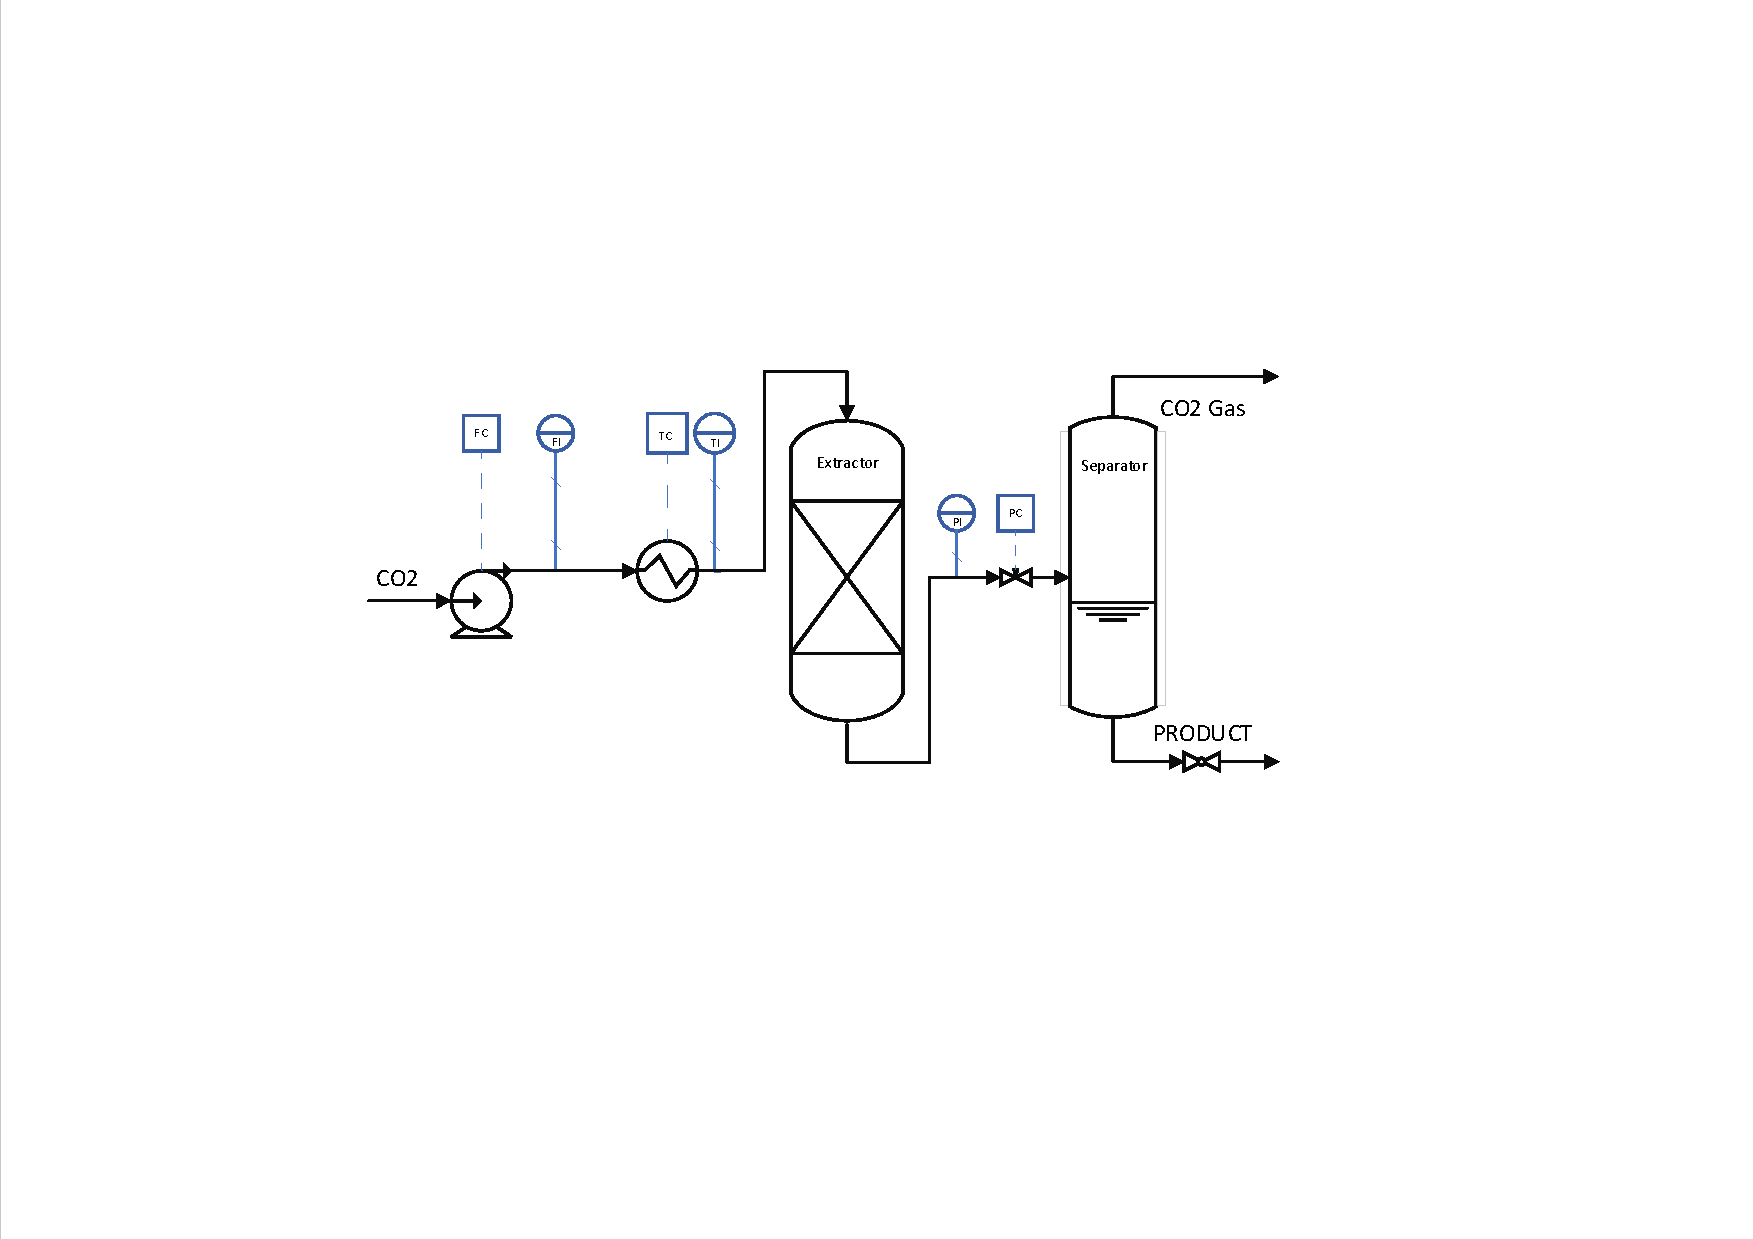
\includegraphics[trim = 6cm 7.5cm 8cm 6cm, clip, width=\linewidth]{Figures/SFE_PFD.pdf}
	\caption{Process flow diagram for solid-fluid extraction process}
	\label{fig: SFE_drawing}
\end{figure}

\subsection{Extraction model} \label{CH: Extraction_model}

\sout{The main components of the model are three one-dimensional differential equations related to mass balances (solid and fluid phase) and heat balance. As in all batch processes, our system has only one steady state. The steady-state occurs only if the solute is entirely taken out of the biomass.

The extraction from a fixed bed is an unsteady process, implying that the solute concentrations in the solid and solvent phases vary over time and space. The convection and the diffusion of the mass and the heat are considered only in the axial direction. The radial distribution of such properties like a velocity is assumed to be flat in that direction. The assumption of the flat velocity profile allows considering a lack of back mixing. The pressure drop in the bed is assumed to be assumed to negligible. Under such conditions, the fluid flow can be considered a plug flow.

Since the solute is assumed to be a single pseudo-component, there is only one mass balance equation for each phase (Eq. s \ref{Model_fluid} and \ref{Model_solid}). On the other hand, there is only one heat balance (Eq.  \ref{Model_heat}) because the presence of a single pseudo-phase is assumed.

Moreover, the process model does not consider the change of particle size or the void fraction during the process. The particles are assumed to be uniformly distributed along the bed and to have the same size.}

{\color{blue}A distributed-parameter model, based on \citet{Reverchon1996}, is used to describe the solid-fluid extraction process. The process model consists of three partial differential equations: two mass balance equations relative to the concentration of solute in the fixed solid phase and the mobile fluid phase, and the heat balance equation relative to the temperature of the fluid phase. The amount of solute in the solvent is considered negligible. Therefore, the fluid phase can be described as pseudo-homogenous, and its properties are assumed to be the same as the solvent.
	
The movement of the mobile pseudo-homogeneous phase (Eq. \ref{Model_fluid}) is considered only in the axial direction. The properties of the system in the radial direction is assumed to be uniform. In addition, it is considered that the boundary layer adjacent to the inner wall of the extractor does not exist. Therefore, the velocity profile is constant across any cross-section of the extractor perpendicular to the axial direction. As a result, the plug flow model can be introduced. The particle size distribution and the void fraction of the solid phase are assumed to be uniform in space and remain constant in time. Moreover, the pressure is considered to be constant along the fixed bed. The mass balance for the fluid phase consists of convection, diffusion, and kinetic terms.
	
Considering the solid phase to be fixed, the convection and diffusion terms in the corresponding mass balance are both assumed to be negligible or absent. Therefore, the mass balance for the solid phase (Eq. \ref{Model_solid}) consists of the kinetic term only. 
	
As for the mass transfer from the solid to the fluid phase, a kinetic term based on two-film theory for the solute is considered. The mass transfer kinetic (Eq. \ref{Model_kinetic_basic}) consists of the overall diffusion coefficient and the concentration gradient, which acts as a driving force for the process. A single pseudo-component is used to represent the extract collectively.
	
The heat balance (Eq. \ref{Model_heat}) consists of the convective and diffusive terms. It follows the assumption of a pseudo-homogeneous phase, which properties are the mean between fluid and solid phases. We consider no heat loss through the wall, and there is no heat generation in the system. Therefore, the temperature of the extractor can be changed only by manipulating the temperature of the inlet stream $T_{In}(t)$.
}

For the sake of clarity of the process model, different colors have been used in the equations to indicate: 
{\color{red}control variables},
{\color{blue}state variables},
{\color{orange}variables} and
{\color{magenta}parameters}.

\subsubsection{Mass balance for the fluid phase} \label{CH: Mass_balance_fluid}
The fluid phase is a mobile phase, which means that the fluids mass balance (Eq. \ref{Model_fluid}) is made of convection, diffusion, and mass transfer kinetic terms.

{\footnotesize
		\begin{align} 
			\label{Model_fluid}
			\cfrac{\partial {\color{blue}c_f}(t,z)}{\partial t} &	=  \underbrace{-\cfrac{1}{ {\color{magenta}\varepsilon A}}\cfrac{{\color{red}F}(t)}{{\color{orange}\rho_f}\left[{\color{blue}T}(t,z),{\color{red}P}(t)\right]} \cfrac{\partial {\color{blue}c_f}(t,z)}{\partial {\color{blue}z}}}_{\text{Convective term}} \\
			&+ \underbrace{ {\color{orange}D^M_e}\left[{\color{blue}T}(t,z),{\color{red}P}(t),{\color{red}F}(t)\right] \cfrac{\partial^2 {\color{blue}c_f}(t,z)}{\partial {\color{blue}z^2}} }_{\text{Diffusive term}} 
			+ \underbrace{ \cfrac{1-{\color{magenta}\varepsilon}}{{\color{magenta}\varepsilon}} {\color{blue}r_e}(t,z) }_{\text{Kinetic term}} 
		\end{align} }

where ${\color{blue}c_f}(t,z), {\color{blue}c_s}(t,z), {\color{blue}T}(t,z)$ correspond to concentration of solute in the fluid phase, concentration of solute in the solid phase and the temperature, respectively. ${\color{blue}r_e}(t,z)$ is a mass transfer kinetic term. ${\color{red}F}(t)$ is the mass flow rate, ${\color{red}P}(t)$ is the pressure, ${\color{magenta}\epsilon}$ is the void fraction of the bed, ${\color{magenta}A}$ is the extractor’s cross section, ${\color{orange}\rho}({\color{blue}T}(t,z),{\color{red}P}(t))$ is the fluid's density, ${\color{magenta}\rho_s}$ is the solids density, ${\color{orange}D^M_e}({\color{blue}T}(t,z),{\color{red}P}(t),{\color{red}F}(t))$ is the axial mass diffusion coefficient.

\subsubsection{Mass balance for the solid phase} \label{Mass_balance_solid}
The solid phase is a stationary phase, which indicates a lack of convection and diffusion terms in the mass balance (Eq.  \ref{Model_solid}). Therefore, the only term present in this equation is the kinetic term (defined as presented in equation \ref{Model_kinetic_basic}), which links solid and fluid phases.

{\footnotesize
		\begin{equation} 
			\label{Model_solid}
			%		{\scriptsize\begin{align*}
			\cfrac{\partial {\color{blue}c_s}(t,z)}{\partial t} = \underbrace{ {\color{blue}r_e}(t,z) }_{\text{Kinetics}}
		\end{equation} }
	
\subsubsection{Kinetic term} \label{CH: Kinetic}
As the solvent flows through the bed, \sout{it forms a film around the porous solid particle and occupies its pores.} {\color{blue}the $CO_2$ molecules diffuse into the pores and adsorb on the particle surface to for an external fluid film around the solid particles through the solvent–solid matrix interactions. Assuming that the mean free path of the molecule is much smaller than the pore diameter, the effect of Knudsen diffusion is small and can be neglected. In this work, the molecular diffusion is assumed.}. The dissolved solute diffuses from the particle's core through the solid-fluid interface, the pore, and the film into the bulk. The graphical representation of the mass transfer mechanism is shown in Figure \ref{fig: SFE_Mechanism}. The mean solute concentration in the solid phase is denoted as ${\color{blue}c_s}$. At the solid-fluid interface, the equilibrium concentrations are given as ${\color{blue}c_s^*}$ and ${\color{blue}c_P^*}$, respectively for solid and fluid phases. The concentration of the solutes in the fluid phase in the centre of the pore is denoted as ${\color{blue}c_{P}}$. As the solute diffuses through the pore, its concentration changes and reaches ${\color{blue}c_{Pf}}$ at \sout{the end} {\color{blue}the opening} of the pore. The solute diffuses through the film around the particle and reaches a concentration in the bulk ${\color{blue}c_f}$. It can be assumed that the two-film theory describes the solid-fluid interface inside the pore. The overall mass transfer coefficient can be introduced if the relation between the solute concentration in one phase and its equilibrium concentration is known.

\begin{figure}[h!]
	\centering
%	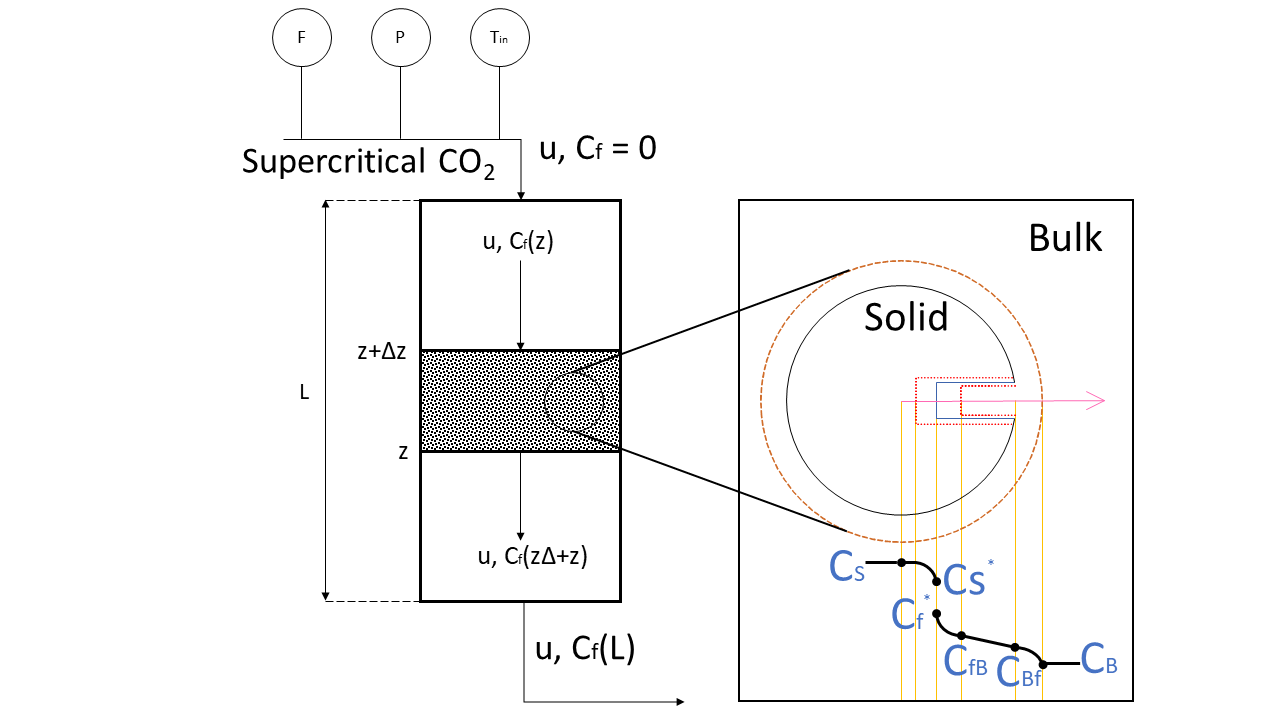
\includegraphics[trim  = 6cm 0cm 3cm 0cm,clip,width=\linewidth]{Figures/SFE_draft.png}
	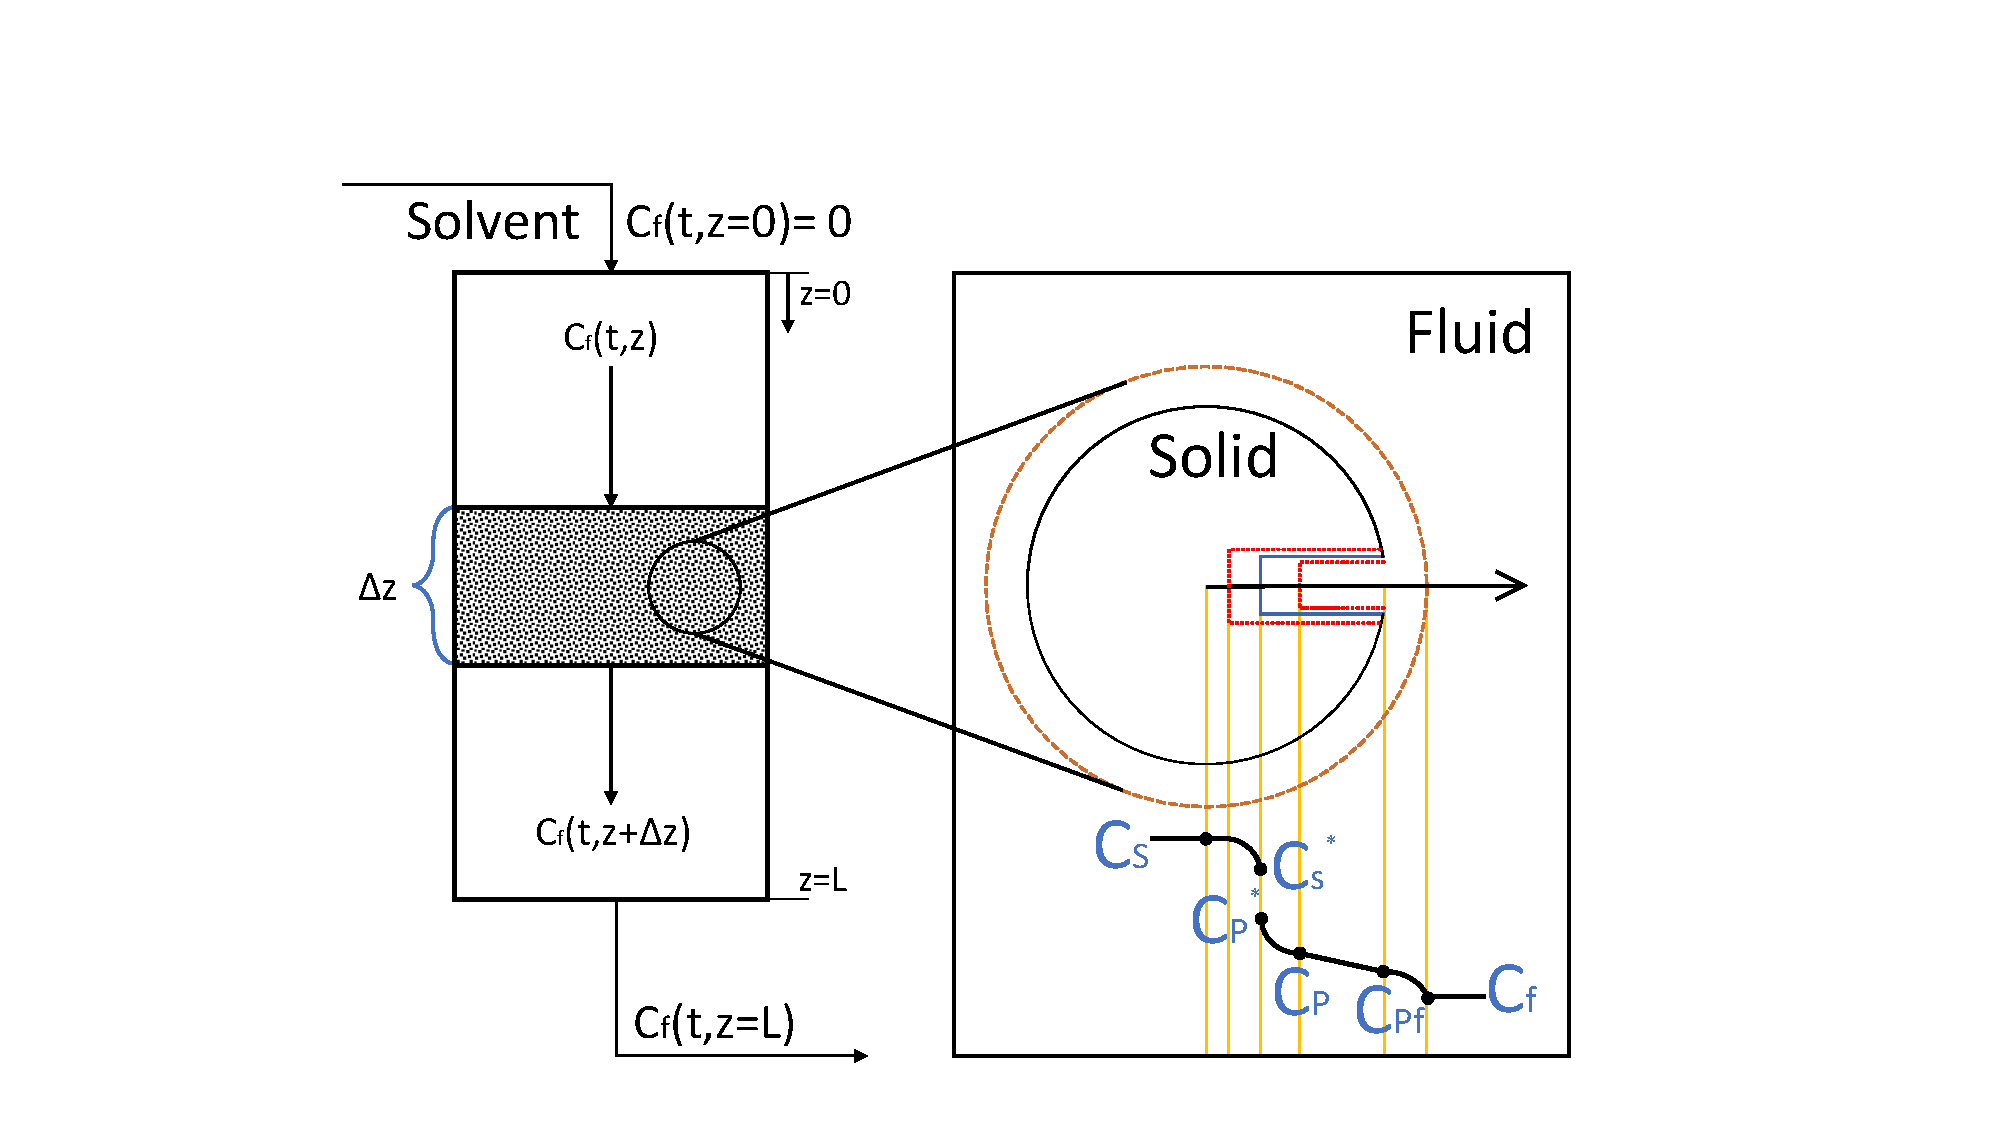
\includegraphics[trim = 5.8cm 1.1cm 6cm 0.8cm,clip,width=1.0\linewidth]{Figures/SFE_draft.pdf}	
	\caption{The extraction mechanism}
	\label{fig: SFE_Mechanism}
\end{figure}

\citet{Bulley1984} suggest a process where the driving force for extraction is given by the difference between concentration of the solute in the bulk, ${\color{blue}c_f}$, and in the centre of the pore, ${\color{blue}c_P^*}$. The concentration ${\color{blue}c_P^*}$ is in equilibrium with ${\color{blue}c_s}$ according to an equilibrium relationship. The rate of extraction is thus ${\color{blue}r_\text{e}}\left({\color{blue}c_f} - {\color{blue}c^*_P}({\color{blue}c_s})\right)$. 

On the other hand, \citet{Reverchon1996} proposes a driving force given by the difference between ${\color{blue}c_s}$ and ${\color{blue}c_P^*}$. ${\color{blue}c_P^*}$ is determined by an equilibrium relationship with ${\color{blue}c_f}$ and the extraction rate is ${\color{blue}r_\text{e}}\left({\color{blue}c_s} - {\color{blue}c^*_P}({\color{blue}c_f})\right)$.

\sout{The kinetic term, denoted as equation \ref{Model_kinetic_basic}, corresponds to a solute transfer rate between both phases. This term is made of the overall diffusion coefficient and the concentration gradient (between one phase and its equilibrium concentration), which acts as a driving force for the process.} {\color{blue}The mass transfer kinetic (Eq. \ref{Model_kinetic_basic}) describes a diffusion rate of the solute from solid particles to the solvent. The kinetic term consists of the overall diffusion coefficient and the concentration gradient, which acts as a driving force for the process.} Based on the work of \citet{Bulley1984}, \citet{Reverchon1996} proposed to define the kinetic terms as

{\footnotesize
\begin{equation} \label{Model_kinetic_basic}
	{\color{blue}r_e}(t,z) = \cfrac{{\color{orange}D_i}({\color{blue}T}(t,z))}{{\color{magenta} \mu l^2} }\left({\color{blue}q}(t,z) - {\color{blue}q^*}(t,z) \right)
\end{equation} }

where ${\color{orange}D_i}({\color{blue}T}(t,z))$ corresponds to the overall diffusion coefficient and ${\color{blue}q^*}(t,z)$ is a concentration at the solid-fluid interface (which according to the internal resistance model is supposed to be at equilibrium with the fluid phase). ${\color{blue}q^*}(t,z)$ can be calculated based on the equilibrium relationship (Eq.  \ref{Linear_equilibirum}). 

\sout{The kinetic term of the model takes into account the properties of the biomass like a sphericity (through the shape coefficient ${\color{magenta}\mu}$ equal to $1/3$ for slabs and $3/5$ for spheres), a characteristic dimension of particles (through the parameter ${\color{magenta}l} = {\color{magenta}r}/3$ where ${\color{magenta}r}$ is the mean particle radius), and the solid density ${\color{magenta}\rho_s}$. The fixed bed is characterized by a void fraction ${\color{magenta}\epsilon}$. }

{\color{blue} The kinetic term of the model takes into account properties of the solid particles like a sphericity (through the shape coefficient ${\color{magenta}\mu}$), a characteristic dimension of particles (through the parameter ${\color{magenta}l} = {\color{magenta}r}/3$ where ${\color{magenta}r}$ is the mean particle radius), and the bulk density ${\color{magenta}\rho_s}$. The fixed bed is characterized by a void fraction ${\color{magenta}\epsilon}$. }

According to \citet{Bulley1984}, a linear equilibrium relationship (Eq.  \ref{Linear_equilibirum}) can be used to find an equilibrium concentration of the solute in the fluid phase ${\color{blue}c_f^*}(t,z)$ is based on concentration of the solute in the solid phase ${\color{blue}c_s}(t,z)$ 

{\footnotesize
\begin{align} \label{Linear_equilibirum}
	{\color{blue}c}(t,z) &= {\color{orange}k_p}({\color{blue}T}(t,z),{\color{red}P}(t)) \allowbreak {\color{blue}q^*}(t,z)
\end{align} }

The volumetric partition coefficient ${\color{orange}k_p}({\color{blue}T}(t,z),{\color{red}P}(t))$ behaves as an equilibrium constant between the solute concentration in one phase and the corresponding equilibrium concentration at the solid-fluid interphase. \sout{ The ${\color{orange}k_p}({\color{blue}T}(t,z),{\color{red}P}(t))$ can be expressed as mass partition factor ${\color{orange}k_m}({\color{blue}T}(t,z))$ according to $\citet{Spiro2007}$ .}
{\color{blue} According to \citet{Spiro2007}, the term ${\color{orange}k_p}({\color{blue}T}(t,z),{\color{red}P}(t))$ can be expressed as the function of mass partition factor ${\color{orange}k_m}({\color{blue}T}(t,z))$ } 

{\footnotesize
\begin{align}
	{\color{orange}k_m}({\color{blue}T}(t,z)) = \cfrac{{\color{orange}k_p}({\color{blue}T}(t,z),{\color{red}P}(t)) {\color{magenta}\rho_s}}{{\color{orange}\rho}({\color{blue}T}(t,z),{\color{red}P}(t))}
\end{align} }

Equation \ref{Model_kinetic} is the full representation of the kinetic term.

{\footnotesize
	\begin{align}
		\label{Model_kinetic}
		{\color{blue}r_e}(t,z) = -\cfrac{{\color{orange}D_i}({\color{blue}T}(t,z))}{{\color{magenta} \mu l^2} }\left({\color{blue}q}(t,z) - \cfrac{{\color{magenta}\rho_s}}{{\color{orange}k_m}({\color{blue}T}(t,z)){\color{orange}\rho}({\color{blue}T}(t,z),{\color{red}P}(t))}  {\color{blue}c}(t,z) \right)
\end{align} }

\subsubsection{Heat balance} \label{CH: heat_balance}
\sout{The heat balance equation (Eq.  \ref{Model_heat}) was developed, assuming the existence of a pseudo-homogeneous phase, which properties are the mean between fluid and solid phases (the amount of solute is considered small enough not to affect the overall heat balance). Equation \ref{Model_heat} contains the convection and the diffusion terms. It is considered that there is no heat loss through the wall, and there is no heat generation in the system. The temperature of the extractor can be changed only by increasing the temperature of the inlet stream. The pseudo-homogenous phase is assumed to flow only in the axial direction. 
The numerator of the factor in front of the convection term of the heat equation contains only the specific heat of the fluid ${\color{orange}C_p}({\color{blue}T}(t,z),{\color{red}P}(t))$ because the solid phase is stationary. Therefore, this factor can be understood as the fraction of the fluid's total heat through convection. On the other hand, the axial heat diffusion is calculated based on the definition of thermal diffusivity for the fluid, as explained in the appendix. }

{\color{blue} The heat balance (Eq. \ref{Model_heat}), is based on \citet{Srinivasan2012}, and consists of convective and diffusive terms. It follows the assumption of a pseudo-homogeneous phase, which properties are the mean between fluid and solid phases. It is considered that there is no heat loss through the walls, and there is no heat generation in the system. The temperature of the extractor can be changed only by manipulating the temperature of the inlet stream ${\color{red}T_{Inlet}}(t)$.
	}

{\footnotesize
	\begin{equation} \label{Model_heat}
		\begin{split}
			\cfrac{\partial {\color{blue}T}(t,z)}{\partial t} &= 
			\underbrace{ -\cfrac{{\color{red}F}(t) {\color{orange}C_p}({\color{blue}T}(t,z),{\color{red}P}(t))}{{\color{magenta}A} 	[(1-{\color{magenta}\epsilon}){\color{orange}\rho}({\color{blue}T}(t,z),{\color{red}P}(t)) {\color{orange}C_p} ({\color{blue}T}(t,z),{\color{red}P}(t)) + {\color{magenta} \epsilon \rho_s C_{ps} } ]} \cfrac{\partial {\color{blue}T}(t,z)}{\partial {\color{blue}z}}  }_{\text{Convection}} + \\
			& + \underbrace{ {\color{orange}D^T_e}({\color{blue}T}(t,z),{\color{red}P}(t)) \cfrac{\partial^2 {\color{blue}T}(t,z)}{\partial {\color{blue}z^2}} }_{\text{Diffusion}}
		\end{split}
	\end{equation} }

where $ {\color{orange}D^M_e}({\color{blue}T}(t,z),{\color{red}P}(t),{\color{red}F}(t))$ is the axial mass diffusion coefficient, ${\color{orange}C_p}({\color{blue}T}(t,z),{\color{red}P}(t))$ is the fluid's specific heat, ${\color{magenta}C_{ps}}$ is the specific heat of the solid phase, ${\color{orange}D^T_e}({\color{blue}T}(t,z),{\color{red}P}(t),{\color{red}F}(t))$ is the axial heat diffusion coefficient.

\subsubsection{Extraction yield} \label{CH: Yield}
\sout{The efficiency of the process (the yield) is calculated according to equation \ref{Model_measurment}. The yield is defined as the ratio between a difference of initial solute's mass in the solid phase ${\color{magenta}m_0}$, and an actual amount of solute in the same phase ${\color{blue}m}$, compared to the initial amount of the solute in the fixed bed ${\color{magenta}m_0}$. The yield can also be calculated based on the change of solutes concentration in the solid phase if the volume of the extractor ${\color{magenta}V}$ is constant.
An output function ${\color{blue}y}(t)$ returns a yield curve that represents the fraction of the solute's mass over time. The yield is obtained by function ${\color{blue}g}({\color{blue}q}(t,z))$. Function ${\color{blue}g}({\color{blue}q}(t,z))$ corresponds to a 'measurement device' that allows to calculate the yield based on the state variable ${\color{blue}q}(t,z)$. }
{\color{blue}The efficiency of the process (the yield) is calculated according to Eq. \ref{Model_measurment}, and is based on the change of solute's mass in the solid phase. It is defined as ratio the ratio between the difference of its initial value ${\color{magenta}m_0}$ and the actual value ${\color{blue}m}(t,z)$, compared to the initial one. The yield can also be calculated based on the change of solutes concentration in the solid phase if the volume of the extractor ${\color{magenta}V}$ is constant.}


{\footnotesize
	\begin{align} 
		\label{Model_measurment}
		{\color{blue}y}(t) ={\color{blue}g}({\color{blue}q}(t,z)) &= \cfrac{ \left({\color{magenta}m_0} - {\color{blue}m}({\color{blue}q}(t,z)) \right) }{{\color{magenta}m_0}} = \cfrac{ {\color{magenta}V} \left({\color{magenta}q_0} - {\color{blue}q}(t,z) \right) }{{\color{magenta}V q_0}} 
	\end{align}	}

\sout{where ${\color{blue}q}(t,z)$ is concentration of solute in a solid phase and a temperature, respectively. ${\color{magenta}m_0}$ is a initial mass of the solute in the solid phase, ${\color{magenta}q_0}$ is a  initial concentration of the solute in the solid phase, ${\color{magenta}V}$ is an extractor volume.}
	
\subsubsection{Dependencies} \label{CH: Dependencies}
{\color{blue}The Peng-Robinson equation of state is used to describe the thermodynamics of the fluid phase. The thermal properties of the pseudo-homogeneous phase are assumed to vary along the extractor, though always remaining equal to the corresponding mean values between the fluid and solid phase. }

In the process model, properties of the supercritical fluid such as the density ${\color{orange}\rho} ({\color{blue}T}(t,z),{\color{red}P}(t))$, the specific heat ${\color{orange}C_p}({\color{blue}T}(t,z),{\color{red}P}(t))$, the thermal conductivity ${\color{orange}k^T}({\color{blue}T}(t,z),{\color{red}P}(t))$, or the viscosity ${\color{orange}\eta}({\color{blue}T}(t,z),{\color{red}P}(t))$ are calculated based on the local temperatures along the fixed bed and the pressure. The Peng-Robinson equation of state is used to find values of a ${\color{orange}\rho} ({\color{blue}T}(t,z),{\color{red}P}(t))$ and ${\color{orange}C_p}({\color{blue}T}(t,z),{\color{red}P}(t))$.

The inter-particle diffusion coefficient ${\color{orange}D^M_e}(\allowbreak{\color{blue}T}(t,z),{\color{red}P}(t),{\color{red}F}(t))$ is calculated from the empirical correlation, as the function of the Reynolds number ${\color{orange}R_e}({\color{blue}T}(t,z),{\color{red}P}(t),\allowbreak{\color{red}F}(t))$ and the Peclet's number ${\color{orange}P_e}({\color{blue}T}(t,z),\allowbreak{\color{red}P}(t),{\color{red}F}(t))$.
The values of the internal diffusion ${\color{orange}D_i} ({\color{blue}T}(t,z))$ and the partition coefficient ${\color{orange}k_m} ({\color{blue}T}(t,z))$ come from the laboratory experiments. The expressions and the detailed information of the parameter fitting can be found in the appendix.

\subsubsection{State-space representation} \label{CH: State_space}
It is assumed that the solvent is free of solute at the entrance of the extractor and that all the solid particles have the same initial solute content ${\color{magenta}q_0}$. Moreover, it is considered that the initial temperature of the extractor in every place is equal to ${\color{magenta}T_0}$. Therefore, the initial conditions employed in the simulation are:

{\footnotesize
\begin{subequations}
	\begin{align*}
		{\color{blue}c}(t = 0, z) &= 0   \\
		{\color{blue}q}(t = 0, z) &= {\color{magenta}q_0} \\
		{\color{blue}T}(t = 0, z) &= {\color{magenta}T_0}
	\end{align*}
\end{subequations} }

The process model can be written in a general form:

{\footnotesize
\begin{align}
	\begin{bmatrix}
		\cfrac{\partial {\color{blue}c}(t,z)}{\partial t}\\
		\cfrac{\partial {\color{blue}q}(t,z)}{\partial t}\\
		\cfrac{\partial {\color{blue}T}(t,z)}{\partial t} 
	\end{bmatrix}
	& =
	\begin{bmatrix}
		{\color{blue}\phi_1} \left( {\color{blue}c}(t,z),{\color{blue}q}(t,z),{\color{blue}T}(t,z); {\color{magenta}\theta} \right)\\
		{\color{blue}\phi_2} \left( {\color{blue}c}(t,z),{\color{blue}q}(t,z),{\color{blue}T}(t,z); {\color{magenta}\theta} \right)\\
		{\color{blue}\phi_3} \left( {\color{blue}c}(t,z),{\color{blue}q}(t,z),{\color{blue}T}(t,z); {\color{magenta}\theta} \right)
	\end{bmatrix} = {\color{blue}\phi} \left( t,z; {\color{magenta}\theta} \right) = \cfrac{\partial {\color{blue}\chi}(t,z)}{\partial t}
\end{align} }

where ${\color{magenta}\theta}$ is a set of parameters present in the model, ${\color{blue}\phi}$ is a set of functions that correspond to state equations of the model, and ${\color{blue}\chi}$ is the state-space model.

The method of lines is used to transform the process model equations into a set of ODEs denoted as ${\color{blue}G}({\color{blue}x}(t);{\color{magenta}p})$. The partial derivatives in $z$-direction are computed using a first-order and second-order finite difference approximation. The backward finite difference is used to approximate first-order derivative, while the central difference scheme is used to approximate second-order derivative. The length of the fixed bed is divided into $N_z$ equally distributed points in $z$-direction. Each function ${\color{blue}\phi_i}$ is transformed to a corresponding set of $N_z$ discretized equations denoted as ${\color{blue}G}_{i\times N_z+1}$ to ${\color{blue}G}_{(i+1)\times N_z}$, where $i$ corresponds to the process model equation. The state-space model ${\color{blue}\chi}(t,z)$ after the discretization is represented by $\dot{{\color{blue}x}}(t)$ (Eq.  \ref{discretization}).

{\footnotesize
\begin{align*} \label{discretization}
	\dot{{\color{blue}x}}(t) &= \cfrac{d {\color{blue}x}(t)}{d t} = 
	\begin{bmatrix}
		\cfrac{d {\color{blue}c_{f,1}}(t)}{d t} 	  \\
		\vdots					  \\
		\cfrac{d {\color{blue}c_{f,N_z}}(t)}{d t} \\
		\\ \hline \\
		\cfrac{d {\color{blue}c_{s,1}}(t)}{d t} 	  \\
		\vdots					  \\
		\cfrac{d {\color{blue}c_{s,N_z}}(t)}{d t} \\
		\\ \hline \\
		\cfrac{d {\color{blue}T_1}(t)}{d t} 	  \\
		\vdots 					  \\
		\cfrac{d {\color{blue}T_{N_z}}(t)}{d t}
	\end{bmatrix}
	=
	\underbrace{\begin{bmatrix}
			{\color{blue}G_1} \left( {\color{blue}x}(t),{\color{blue}q}(t),{\color{blue}T}(t); {\color{magenta}p} \right)\\ 
			\vdots\\ 
			{\color{blue}G_{N_z}} \left( {\color{blue}c}(t),{\color{blue}q}(t),{\color{blue}T}(t); {\color{magenta}p} \right)\\ 
			\\ \hline \\ \\
			{\color{blue}G_{N_z+1}} \left( {\color{blue}c}(t),{\color{blue}q}(t),{\color{blue}T}(t); {\color{magenta}p} \right)\\ 
			\vdots\\
			{\color{blue}G_{2N_z}} \left( {\color{blue}c}(t),{\color{blue}q}(t),{\color{blue}T}(t); {\color{magenta}p} \right)\\ 
			\\ \\ \hline \\ 
			{\color{blue}G_{2N_z+1}} \left( {\color{blue}c}(t),{\color{blue}q}(t),{\color{blue}T}(t); {\color{magenta}p} \right) \\
			\vdots\\
			{\color{blue}G_{3N_z}} \left( {\color{blue}c}(t),{\color{blue}q}(t),{\color{blue}T}(t); {\color{magenta}p} \right)
	\end{bmatrix}}_{{\color{blue}G} \left( {\color{blue}x}(t); {\color{magenta}p} \right)} 
\end{align*} }

where ${\color{blue}x} \in \mathbb{R}^{N_x = 3N_z} $ and ${\color{magenta}p} \in \mathbb{R}^{N_p =  N_{\theta} + N_u } $, $N_{\theta}$ is the number of model parameters, $N_{u}$ is the number of control variables.

{\color{blue} In a state-space sense, the state variables of the system are the local concentrations of solute in the fluid and solid phases ($c(t,z)$ and $q(t,z)$, respectively), and the local temperature of the pseudo-homogeneous phase ($T(t,z)$). The controllable input variables are the mass flow-rate and temperature of the solvent in the feed ($F_\text{in}(t) = F(t)$ and $T_\text{in}(t) = T(t,z=0)$, respectively) and the pressure in the extractor ($P(t,z) = P(t)$). {\color{red}We also assume that extraction yield can be modelled as a function of a known initial mass of solute in the solid phase and it can be measured after the separator ($Y(t)$).} The system is controllable by manipulating the flow-rate and temperature of CO2 in the feed, and the pressure in the extractor. }

\newpage
\section{Bayes theorem} \label{CH: Bayes}

As discussed by \citet{Himmelblau1970}, The Bayesian approach to estimation make use of prior information. Such prior knowledge can come from theoretical considerations, from the results of previous experiments, or from assumptions by the experimenter. Typically, a Bayesian approach assumes a prior probability distribution of an unknown parameter $\theta$ in some parameter space $\boldsymbol{\theta}$. The distribution is updated by using Bayes' rule to obtain the posterior probability distribution. 

Consider a set of events or outcomes, $A_1,A_2,...,A_n$, and some other event $B$. Bayes' theorem states that the probability that event $A_i$ will occur, given that event $B$ has already occured, which will denoted by $P\{A_i|B\}$, is equal to the product of the probability that $A_i$ will occur regardless of whether $B$ will take place and the probability that $B$ will occur, given that $A_i$  has already taken place, divided by the probability of the occurrence of $B$:

\begin{equation}
	P\{A_i|B\} = \cfrac{P\{B|A_i\}P\{A_i\}}{P\{B\}}
\end{equation}

Further, if al events comprising the set $\{A_i\}$ are included in $A_1,A_2,...,A_n$, then

\begin{equation} \label{EQ: Bayes_discrit}
	P\{A_i|B\} = \cfrac{P\{B|A_i\}P\{A_i\}}{ \sum_{i=1}^{n} P\{B|A_i\} P\{A_i\} }
\end{equation}

We can interpret these symbols as follows:

\begin{enumerate}
	\item $P\{A_i\}$ is a measure of our degree of belief that event $A_i$ will occur or that hypothesis $A_i$ is true prior to the acquisition of additional evidence that may alter the measure. $P\{A_i\}$ is denoted the \textit{prior probability}.
	\item $P\{A_i|B\}$ is a measure of our degree of belief that event $A_i$ will occur or that hypothesis $A_i$ is true, given additional evidence $B$ pertinent ot the hypothesis. $P\{A_i|B\}$ is termed the \textit{posterior probability}.
	\item $P\{B|A_i\}$ denotes the likelihood that event $B$ will occur, given that event $A_i$ is true. $P\{B|A_i\}$ is a conditional probability, interpreted in the Bayesian framework as a likelihood, $L(A_i|B)$.
\end{enumerate}

For continuous variable, Bayes' theorem can be more conveniently expressed in terms of the probability density function rather than the probabilities themselves. Equation \ref{EQ: Bayes_discrit} can be expressed in terms of a set of observed values of the random variable $X$, \textbf{x} and unknown parameter $(s)\theta$ as

\begin{equation} \label{EQ: Bayes_continous}
	p\left( \theta|X=\textbf{x} \right) = p\left( \theta|\textbf{x} \right) = \cfrac{L\left( \theta|\textbf{x} \right) p(\theta)}{\int_{-\infty}^{+\infty} L\left( \theta|\textbf{x} \right) p(\theta) d\theta}
\end{equation}

where

$p(\theta|\textbf{x}) = ~$the posterior probability density function for $\theta$; it includes knowledge of the possible values of $\theta$ gained from the experimental data \textbf{x}

$p(\theta) = ~$ the prior probability density function for $\theta$ (before the experiment in which \textbf{x} was observed)

$L\left( \theta|\textbf{x} \right) = p\left( \textbf{x}|\theta \right) = ~$ the probability density function termed the likelihood function of $\theta$ given \textbf{x}

The denominator in Equation \ref{EQ: Bayes_continous} is a normalizing factor chosen so that the integration of the posterior distribution is unit, i.e., $\int_{-\infty}^{+\infty} p\left( \theta|\textbf{x} \right) = 1$. By taking into account the law of total probability, the denominator can be written as

\begin{equation}
	\int_{-\infty}^{+\infty} p\left( \textbf{x}|\theta \right) p(\theta) d\theta = p(\textbf{x})
\end{equation}

If the prior distribution is a uniform distribution, that is the prior distribution is a constant, the \ref{EQ: Bayes_continous} reduces to 

\begin{equation}
	p\left( \theta|\textbf{x} \right) = \cfrac{L\left( \theta|\textbf{x} \right)}{\int_{-\infty}^{+\infty} L\left( \theta|\textbf{x}\right) d\theta}
\end{equation}

If the prior knowledge concerning a postulated event or hypothesis is poor, the posterior probability is largely or entirely determined by the likelihood function, that is, by the additional accumulated evidence for which the likelihood function acts as a mathematical expression. If prior knowledge outweighs recent evidence, however, then the posterior probability is determined almost solely by the prior probability.

In the application of tests and the design of experiments, certain definitions and rules concerning probability are needed and are listed below.

\begin{enumerate}
	\item It follows from the frequency theory of probability that: $0 \leq P \leq 1$
	\item If the probability of occurrence of one event $A$ depends on whether or not event $B$ has occurred, the two events are termed \textit{dependent}; if the probability of occurrence of event $A$ does not depend on the occurrence of $B$, or the reverse, the two events are \textit{independent}.
	\item \textbf{Addition Rule}
	If $A_1,A_2,...,A_n$ are mutually exclusive events, i.e., cannot occur at the same time, the probability of occurrence of just one of the events is equal to the sum of the probabilities of each $A_i$:
	
	\begin{equation}
		P\left( A_1, \text{or~} A_2,..., \text{or~} A_n \right) = \sum_{i=1}^{n} P\left( A_i \right)
	\end{equation}

	Very often we let
	\begin{equation}
		\sum_{i=1}^{n} P\left( A_i \right) = 1
	\end{equation}
	
	Also, if each event is equi-probable so that $P(A_i) = q$,
	
	\begin{equation}
		\sum_{i=1}^{n} q = nq = 1 \qquad \text{or} \qquad  q=\cfrac{1}{n} = P\left( A_i \right)
	\end{equation}
	
	In set theory, mutually exclusive event have no points in common. The union of the sets which represents the set of all elements that belong to
	
	\begin{equation}
		P\left( A_1 \cup A_2 \cup ... \cup A_n \right) = P(A_1) + P(A_2) + ... + P(A_n)
	\end{equation}

	\item \textbf{Multiplication Rule}
	If $A$ and $B$ are \textit{independent} event
	
	\begin{equation}
		P\left( A \text{~and~} B\right) = P(A)P(B)
	\end{equation}
	
	In set theory the intersection of $A$ and $B$ is the set of all elements that belong to $A$ and $B$:

	\begin{equation} \label{EQ: Probabiltiy_independet_a}
		P\left( A \cap B  \right) = P(A)P(B)
	\end{equation}

	If the $A$ and $B$ are \textit{dependet} events,
	
	\begin{equation} \label{EQ: Probabiltiy_independet_b}
		P\left(A|B\right) = \cfrac{P\left( A \cap B \right)}{P(B)}
	\end{equation}

	where the symbol $P(A|B)$ means "probability of $A$ given $B$". As a corollary,
	
	 \begin{subequations}
		\begin{alignat}{2}
			P\left( A \cap B \right) &= P(B) P(A|B) \label{EQ: Probabiltiy_dependet_a} \\
			&= P(A)P(B|A) \label{EQ: Probabiltiy_dependet_b}
		\end{alignat}
	\end{subequations}
	
	Two kind of probabilities enter Equation \ref{EQ: Probabiltiy_dependet_a} (or Equation \ref{EQ: Probabiltiy_dependet_b}): the absolute probability of event $B$ (or $A$) irrespective of whether or not $A$ (or $B$) has occurred, and that the conditional probability of event $A$ (or $B$) computed on the assumption that $B$ (or $B$) has occurred. Equation \ref{EQ: Probabiltiy_independet_a} or \ref{EQ: Probabiltiy_independet_b} is special case of Equation \ref{EQ: Probabiltiy_dependet_a} or \ref{EQ: Probabiltiy_dependet_b}, because if the event are independent $P(A|B)=P(A)$.
	For the case of many event, Equation \ref{EQ: Probabiltiy_independet_a} can be expanded to 
	
	\begin{equation}
		\begin{split}
			P(A_1 \text{~and~} A_2 \text{~and~} ... \text{~and~} A_n) &= P(A_1)\cdot P(A_2) \cdot  ...\cdot P(A_n) \\ &= \prod_{i=1}^{n} P(A_i)
		\end{split}
	\end{equation}

	\item Another useful relationship for event which are not mutually exclusive is 
	
	\begin{equation}
		P(A) + P(B) - P(A \cap B) = P(A \cup B)
	\end{equation}
		
\end{enumerate}

\newpage
\section{Parameter estimation} \label{CH: Parameter_estimation}

Conceptually, in the measurement equation the unobservable $\epsilon(t)$ is added to $y(t)$ to give the observable dependent variable $Y(t)$ defined as:

\begin{equation}
	Y(t) = y(t) + \epsilon(t)
\end{equation}

If the estimated parameter $\hat{\alpha}$ replaces the model parameter $\alpha$, the residue error is $\textbf{E} = Y(t) - \hat{Y}(t)$. The objective in parameter estimation is to obtain the "best" estimate of $\alpha$ based on the continuous observations $Y(t)$ or the discrete observations $Y(t_i)$. 

We assume that $x(t)$ is given \textit{a priori} but the $\textbf{y}_0$ and $\alpha$ are to be estimated over the time interval $0 \leq t \leq t_n$ from discrete observation described by the following relation:

\begin{equation}
	\textbf{Y}(t_i) = h(t_i)y(t_i) + \epsilon(t_i) \qquad 1 \leq i \leq n
\end{equation}

where $\textbf{Y}(t_i)$ is an $n \times 1$ column vector, $h(t_i)$ is an $n \times v$ matrix given \textit{a priori}, and $\epsilon (t_i)$ is an $x \times 1$ column vector ("noise" vector) whose elements are the unobservable errors. The above equation can be written in general form as:

\begin{equation} \label{EQ: Measurment_noise}
	\textbf{Y}(t_i) = \Psi(\alpha, y_0, t_i) + \epsilon(t_i)
\end{equation}
where $\Psi$ is the matrix of functions.

Because of the difficulty of obtaining analytical solutions to the deterministic process model, experiments have been arranged wherby the vector of derivatives $d\textbf{Y}/dy$ is measured rather than \textbf{Y} itself. In such cases, it is assumed that the unobservable error is added to the deterministic derivative $dy/dt$ as follows:

\begin{equation}
	\cfrac{d\textbf{Y}}{dt} = \cfrac{dy}{dt} + \epsilon
\end{equation}

\subsection{Least squares estimation}
A least squares parameter estimation does not require prior knowledge of the distribution of unobservable errors, yield  unbiased estimates, that is, $ \mathbb{E}\{\hat{Y}(t) = y(t) \} $, and results in the minimum variance among all linear unbiased estimators. If the observations $\textbf{Y}$ for the model responses are continuous functions of time from $t = 0$ to $t = t_f$, the Markov (or "rigorous least squares") criterion is to minimize:

\begin{equation}
	\phi =  \cfrac{1}{2} \int_{0}^{t_f}  \left[ \textbf{Y} - \Psi \right]^T \Gamma^{-1} \left[ \textbf{Y} - \Psi \right] dt
\end{equation}

where $\Gamma$ is the covariance matrix (or perhaps a matrix of appropriate weights), and $\phi$ is the time integrated value of the error squared ("integral squared error"). If the observations are made at discrete instants of time, $t_i$, $i = 1,2,...,n$, the Markov criterion is to minimize:

\begin{equation}
	\phi = \cfrac{1}{2} \sum_{i=1}^{n} \left[ \textbf{Y}(t_i) - \Psi(t_i) \right]^T \Gamma^{-1} \left[ \textbf{Y}(t_i) - \Psi(t_i) \right] 
\end{equation}

If $\Gamma$ is a diagonal matrix, $\phi$  becomes a "weighted least squares" criterion; if $\Gamma = \sigma^2 \textbf{I}$ where $\sigma$ is a standard deviation, $\phi$ is the "ordinary least squares" criterion.

\subsection{Maximum likelihood estimation}

Maximum likelihood estimation (MLE) is a method of estimating the parameters of an assumed probability distribution, given some observed data. This is achieved by maximizing a likelihood function so that, under the assumed statistical model, the observed data is most probable. The MLE has the desirable characteristics of asymptotic efficiency and normality. Each time it has been associated with the (joint) normal distribution because of mathematical convenience. Consider the joint probability density function (the likelihood function) $p(\alpha, y_0|y(t_1),y(t_2),...,y(t_n))$ for $\alpha$ and $y_0$ if a maximum of this function over all choices of $y_0$ and $\alpha$ can be found, the estimates so obtained are maximum likelihood estimates. The conditions at the maximum can be evolved incorporating prior information as follows.

The posterior probability density $p(\alpha,y_0|y(1),y(2),...,y(t_n))$ can be expressed as the ratio of two probability densities if we make use of the analog for continuous variables of Equation \ref{EQ: Probabiltiy_independet_b}:

\begin{equation} \label{EQ: Posterior_distribution}
	p\left( \alpha,y_0|y(t_n,...,y(1)) \right) = \cfrac{p\left( \alpha, y_0, y(t_n),...,y(t_1) \right)}{p\left( y(t_n),...,y(t_1) \right)}
\end{equation}

The numerator of the right-hand side od Equation \ref{EQ: Posterior_distribution} using Equation \ref{EQ: Probabiltiy_dependet_a} becomes 

\begin{equation}
	\begin{split}
		p\left( \alpha,y_0,y(t_n),...,y(t_1) \right) &= p\left( y(t_n)|\alpha,y0,y(t_{i-1},...,y(t_1)) \right) \\ &\cdot p\left( \alpha,y_0,y(t_{n-1}),...,y(t_1) \right)
	\end{split}
\end{equation}

These operations can be continued repetitively until we get

\begin{equation}
	p\left( \alpha,y_0,y(t_n),...,y(t_1) \right) = p\left( \alpha,y_0 \right) \prod_{i=1}^{n} p\left( \alpha,y_0,y(t_{n-1}),...,y(t_1) \right)
\end{equation}

Examination of Equation \ref{EQ: Measurment_noise} shows that $\textbf{Y}(t_i)$ depends only on $t_i$, $y_0$, $\alpha$ and $\epsilon(t_i)$ and is not conditioned by any previous measurement. Consequently, we can write 

\begin{equation}
	p\left( y(t_i)|\alpha,y_0, y(t_{i-1}),...,y(t_1) \right) = p\left( y(t_i)|\alpha,y_0 \right)
\end{equation}

provided Equation \ref{EQ: Measurment_noise} is observed as a constraint. The desired joint conditional probability function is thus

\begin{equation}
	p\left( \alpha,y_0|y(t_n),...,y(t_1) \right) = \cfrac{p\left( \alpha,y_0 \right) \prod_{i=1}^{n} p\left( y(t_i)|\alpha,y_0 \right) }{p\left( y(t_n),...,y(t_1) \right)}
\end{equation}

The function to be maximized will be the logarithm of the likelihood function $L = p\left( \alpha,y_0, y(t_n),...,y(t_1) \right)$ constrained by equation \ref{EQ: Measurment_noise}, which can be written as $\ln(L)$ plus the Lagrangian multipliers $\lambda(t_k)$ times the constraint function, or

\begin{equation} \label{EQ: MLE_Lagrangian}
	\begin{split}
		L^* \equiv \ln p\left( \alpha,y_0 \right) + \sum_{i=1}^{n} \left\{ \ln p(y(t_i)|\alpha,y_0) \right. \\
		\left. + \lambda^T \cdot \left[ y(t_i) - \Psi\left( \alpha,y_0,t_i \right) - \epsilon(t_i) \right] \right\} \\ - \ln \left[ p\left( y(t_n),...,y(t_1) \right) \right]
	\end{split}
\end{equation}

By assumption of the relation of Equation \ref{EQ: Measurment_noise}

\begin{equation} \label{EQ: Noise_prob}
	p\left( y(t_i) | \alpha,y_0 \right) = p\left( \epsilon(t_i) \right)
\end{equation}

and specially

\begin{equation} \label{EQ: Noise_prob_norm}
	p\left( \epsilon(t_i) \right) = \cfrac{1}{ (2\pi)^{v/2} |\Gamma(t_i)|^{1/2} } \exp \left[ -\cfrac{1}{2}\epsilon(t_i) \left( \Gamma(t_i) \right)^{-1} \epsilon(t_i) \right]
\end{equation}
where $|\Gamma|$ is the det$~\Gamma$, and $\Gamma$ is the covariance matrix of $\epsilon$, i.e., of the response.

After Equation \ref{EQ: Noise_prob} is substituted into Equation \ref{EQ: MLE_Lagrangian}, and $L^*$ is differentiated with respect to each of the estimated and $\epsilon(t_i)$, and the resulting expression is equated to zero, we get

 \begin{subequations} \label{EQ: MLE_Lag_diff}
	\begin{alignat}{2}
		\cfrac{\partial L^*}{\partial y_0} &= \cfrac{\partial}{\partial y_0} \ln p(\alpha,y_0) - \sum_{i=1}^{n} \lambda^T(t_i) \cfrac{\partial}{\partial y_0} \Psi(\alpha, y_0,t_i) = 0^T \\
		\cfrac{\partial L^*}{\partial \alpha} &= \cfrac{\partial}{\partial \alpha} \ln p(\alpha,y_0) - \sum_{i=1}^{n} \lambda^T(t_i) \cfrac{\partial}{\partial \alpha} \Psi(\alpha, y_0,t_i) =0 \\
		\cfrac{\partial L^*}{\partial \epsilon(t_i)} &= \cfrac{\partial}{\partial \epsilon(t_i)} \ln p(\epsilon(t_i)) - \lambda^T(t_i) = 0^T
	\end{alignat}
 \end{subequations}

Substitution of Equation \ref{EQ: Noise_prob_norm} into the last Equation of \ref{EQ: MLE_Lag_diff} makes it possible to solve for $\lambda(t_i)$:

\begin{align}
	\lambda(t_i) &= -\left( \Gamma(t_i) \right)^{-1} \epsilon(t_i) \nonumber \\
	&= -\left( \Gamma(t_i) \right)^{-1} \left[ \textbf{Y}(t_i) - \Psi(\alpha,y_0,t_i) \right]
\end{align}

and to eliminate $\lambda(t_i)$ from the first two equations of \ref{EQ: MLE_Lag_diff}.

For convenience we shall define a new column vector $\alpha^*$ in which all the elements of $\alpha$ are arranged as follows:

\begin{equation}
	\alpha^* = \begin{bmatrix}
		\alpha_{1,1} & \alpha_{1,2} & \cdots & \alpha_{1,v} & \alpha_{2,1} & \cdots & \alpha_{2,v} & \cdots & \alpha_{v,v}
	\end{bmatrix}^T	
\end{equation}

Finally, we assume that $y_0$ and $\alpha^*$ are distributed by a joint normal distribution and that the prior  distribution are, respectively

\begin{subequations} \label{EQ: MLE_Priors}
	\begin{align}
		&p\left( \alpha^* \right) = \cfrac{1}{ (2\pi)^{v/2} |\Omega_{\alpha^*}|^{1/2} } \exp \left[ -\cfrac{1}{2} \left( \alpha^* - \alpha^{*(0)} \right)^T \Omega_{\alpha^*}^{-1} \left( \alpha^* - \alpha^{*(0)} \right) \right] \\
		&p\left( y_0 \right) = \cfrac{1}{ (2\pi)^{v/2} |\Omega_{y_0}|^{1/2} } \exp \left[ -\cfrac{1}{2} \left( y_0 - y_0^{(0)} \right)^T \Omega_{y_0}^{-1} \left( y_0 - y_0^{(0)} \right) \right] 
	\end{align}
\end{subequations}
where $\Omega$'s are the respective covariance matrices for $\alpha^*$ and $y_0$, and the subscript $(0)$ designates the prior estimated of $\alpha^*$ and $y_0$. If we assume that $\alpha^*$ and $y_0$ are independent

\begin{equation}
	\ln p(\alpha^*,y_0) = \ln p(\alpha^*) + \ln p(y_0)
\end{equation}

Introduction of the prior distributions, Equations \ref{EQ: MLE_Priors}, plus the expression for $\lambda(t_i)$ into the first two equations of \ref{EQ: MLE_Lag_diff} gives the final equations from which the estimators of $\alpha^*$ and $y_0$ can be obtained:

\begin{subequations} 
	\begin{align}
	-\left( \hat{y}_0 - y_0^{(0)} \right)^T \Omega_{y_0}^{-1} &+ \sum_{i=1}^{n}\left[ \textbf{Y}(t_i) - \Psi\left( \hat{\alpha}, \hat{y}, t_i \right) \right]^T \Gamma^{-1}(t_i) \nonumber \\ 
	&\cdot \cfrac{\partial}{\partial y_0} \Psi\left( \hat{\alpha}, \hat{y}, t_i \right) = 0^T \\
	-\left( \hat{\alpha}^* - \alpha^{*(0)} \right)^T \Omega_{\alpha^*}^{-1} &+ \sum_{i=1}^{n}\left[ \textbf{Y}(t_i) - \Psi\left( \hat{\alpha}, \hat{y}, t_i \right) \right]^T \Gamma^{-1}(t_i) \nonumber \\ 
	&\cdot \cfrac{\partial}{\partial \alpha^*} \Psi\left( \hat{\alpha}, \hat{y}, t_i \right) = 0^T \nonumber \\
	\end{align}
\end{subequations}
where the overlay caret denotes estimated parameters.

Note that under the assumption that the elements of $\Omega$ are essentially infinite (prior knowledge is diffuse), the elements of $\Omega^-1$ are zero, the equations for the maximum likelihood estimates coincide with those for the least squares estimates, and the same calculations for precision in the estimates apply.

\hrule

For some models, these equations can be explicitly solved for $\hat{\alpha}^*$ and $\hat{y}$ but in general no closed-form solution to the maximization problem is known or available, and an MLE can only be found via numerical optimization. Under the assumption of normality, the lack of prior knowledge about the parameters and known initial conditions, the optimization problem is defined as follow:

\begin{equation}
	\hat{\alpha} = \arg \max_{\alpha \in \Theta} L = \arg \max_{\alpha \in \Theta} p(\alpha|y(t_1),y(t_2),...,y(t_n))
\end{equation}

Intuitively, this selects the parameter values that make the observed data most probable. The specific value $\hat{\alpha}$ that maximizes the likelihood function $L$ is called the maximum likelihood estimate. Further, if the function $\hat{\alpha}:\mathbb{R}\rightarrow\Theta$ so defined is measurable, then it is called the maximum likelihood estimator.

If the random samples $y(t_1)$, $y(t_2)$,...,$y(t_n)$ come from a normal distribution with unknown mean $\hat{\alpha}$ and variance $\sigma^2$, then the joint probability function can be written as 

\begin{equation}
	p(\alpha|y(t_i)) = \cfrac{1}{\sqrt{2\pi\sigma}}\exp\left[-\cfrac{ \left( \textbf{Y}(t_i) - \Psi\left( \hat{\alpha}, \hat{y}, t_i \right) \right)^2}{2\sigma}\right]
\end{equation}

Then the likelihood function is defined as follow:

\begin{multline} 
	L =\prod\limits_{i=1}^n p(\alpha|y(t_i))= \\ \sigma^{-n/2}(2\pi)^{-n/2}\exp\left[-\cfrac{1}{2\sigma}\sum\limits_{i=1}^n \left( \textbf{Y}(t_i) - \Psi\left( \hat{\alpha}, \hat{y}, t_i \right) \right)^2\right]
\end{multline}

By taking the ln of the likelihood function, the final form of a cost function is obtained:

\begin{equation} 
	\ln L=-\cfrac{n}{2}\ln\sigma-\cfrac{n}{2}\ln(2\pi)-\cfrac{\sum\limits_{i=1}^n \left( \textbf{Y}(t_i) - \Psi\left( \hat{\alpha}, \hat{y}, t_i \right) \right)^2}{2\sigma}
\end{equation}

\section{Results} \label{CH: Results}

\section{Conclusions}

% ===================================================
% Bibliography
% ===================================================
%% Loading bibliography style file
\clearpage
%\bibliographystyle{model1-num-names}
\bibliographystyle{unsrtnat}
\bibliography{mybibfile}

\clearpage \appendix \label{appendix}
\section{Appendix} 

\newpage
\begin{table*}[p]
		\caption{Notation}
		\label{tab::symbols}
		\begin{tabular}{ |c|l|c| } 
			\hline
			Symbol 		& 	Description 							& Unit 						\\ \hline
			$A$			&	cross-section							& $m^2$ 					\\ \hline
			$c$			&	concentration in fluid phase			& $kg ~ m^{-3}$				\\ \hline
			$Cp$		&	specific heat of the fluid				& $J ~ mol^{-1} ~ K^{-1}$ 	\\ \hline
			$Cp_s$		&	specific heat of the solid				& $J ~ mol^{-1} ~ K^{-1}$ 	\\ \hline
			$D_e^M$		&	axial mass diffusion coefficient		& $m^2 ~ s^{-1}$			\\ \hline
			$D_e^T$		&	axial heat diffusion coefficient		& $m^2 ~ s^{-1}$			\\ \hline
			$Di$		&	internal diffusion coefficient			& $m^2 ~ s^{-1}$			\\ \hline
			$dp$		&	particle diameter						& $m$						\\ \hline
			$F(t)$		&	mass flow-rate							& $kg ~ s^{-1}$				\\ \hline
			$km$		&	partition coefficient					& $[-]$						\\ \hline
			$k^T$		&	thermal conductivity					& $W ~ m^{-1} ~ K^{-1}$		\\ \hline
			$l$			&	characteristic dimension				& $m$						\\ \hline
			$L$			&	total length of the bed					& $m$						\\ \hline
			$m$			&	mass of the oil in solid phase			& $kg$						\\ \hline
			$m_0$		&	initial mass of the oil in solid phase	& $kg$						\\ \hline
			$M_{CO_2}$	&	molecular mass of CO2					& $mol ~ kg^{-1}$			\\ \hline
			$Np$		&	number of model parameters and control variables & $[-]$			\\ \hline
			$N_{\theta}$&	number of model parameters				& $[-]$						\\ \hline
			$Nu$		&	number of control variables				& $[-]$						\\ \hline
			$Nz$		&	number of grid points in z-direction	& $[-]$						\\ \hline
			$p$			&	vector of model parameters and control variables	& $[-]$			\\ \hline
			$P(t)$		&	pressure								& $bar$						\\ \hline
			$Pe$		&	Peclet's number							& $[-]$						\\ \hline
			$q$			&	concentration in solid phase			& $kg ~ m^{-3}$				\\ \hline
			$R$			&	gas constant							& $J ~ K^{-1} ~ mol^{-1}$	\\ \hline
			$Re$		&	Reynolds number							& $[-]$						\\ \hline
			$t$			&	time									& $s$						\\ \hline
			$T$			&	temperature								& $K$						\\ \hline
			$T_0$		&	initial temperature						& $K$						\\ \hline
			$V$			&	volume of the extractor					& $m^3$						\\ \hline
			$y$			&	yield	 								& $[-]$						\\ \hline
			$z$			&	length									& $m$						\\ \hline
			$Z$			&	compressibility	factor					& $[-]$						\\ \hline
			$\epsilon$	&	void fraction							& $[-]$						\\ \hline
			$\rho$		&	density of the fluid					& $kg ~ m^{-3}$				\\ \hline
			$\rho_s$	&	solid density							& $kg ~ m^{-3}$				\\ \hline
			$\mu$		&	shape coefficient						& $[-]$						\\ \hline
			$\theta$	&	vector of model parameters				& $[-]$						\\ \hline
			$\eta$		&	viscosity								& $cP$						\\ \hline				
						& 											&							\\ \hline			
		 	Subscript	& 											&							\\ \hline
			$0$			&	initial conditions						& $[-]$						\\ \hline
			$^*$		&	equilibrium conditions					& $[-]$						\\ \hline							
		\end{tabular}
\end{table*}
\end{document}